\chapter{Methodology}

\label{chapter:methodology}

\begin{figure}[h]
    \centering
    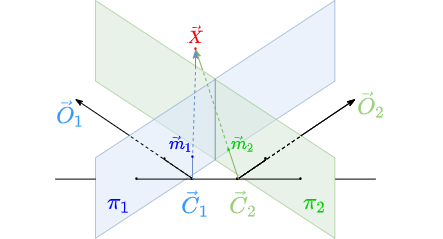
\includegraphics[width=.8\textwidth]{graphics/td90deg.png}
    \caption[The proposed approach model.]{Ilustration of the proposed approach. $\vec{C}_1$, $\vec{C}_2$ are optical centers of two cameras with projection planes $\pi_1$ and $\pi_2$. 
    $\vec{O}_1$ and $\vec{O}_2$ are the corresponding optical axes. The 3D point $\vec{X}$ is in the cameras' overlapping field of view, $\vec{m}_1$ and $\vec{m}_2$ are its projections on corresponding image planes.}
    \label{fig:td90deg}
\end{figure}

The main task of this thesis is to create a compact obstacle avoidance system such that it can be mounted on MAVs with size and weight restrictions.
The proposed method is related to SfM or optical flow algorithms as well as standard stereo matching algorithms.

Firstly, synchronized images from both cameras are captured. Features are detected using the ORB feature extractor \cite{Rublee2011} in the areas of these images that correspond to the overlapping part of their fields of view. 
These features are then matched using the brute-force matcher, described in \autoref{sec:features}.
The 3D position of each of these features relative to the cameras is estimated using a calibrated projection model and known relative transformation between the cameras.
Finally, the obtained 3D positions are the output of this algorithm. 

The quality of the 3D point estimation depends on the cameras' relative transformation, the calibration of their projection model, the keypoint (feature) extractor, and the matcher.
The obtained 3D points can be used to estimate the scale in an SfM algorithm that runs parallel to the described method (refer to  \autoref{fig:intro_general}).
The estimated distance to nearby objects can be used in a feedback loop inside the MAV's control system to correct path planning, considering the obstacles found.

This chapter describes the mathematical model of the problem and all algorithms used in the process: calibration of the projection model, calibration of the relative transformation between the cameras, feature extraction, feature matching, and estimation of the 3D position of the matched features.

\section{Description of the optical setup}

The optical setup assumed by the proposed method is shown in \autoref{fig:td90deg}.
There are two cameras with optical centers at $\vec{C}_1$ and $\vec{C}_2$ with a known static translation $\vec{t}_{21}$ and rotation $\mat{R}_{21}$ between coordinate frames of the cameras.
The rotation represented by $\mat{R}_{21}$ is assumed to be close to a \ang{90} rotation in the epipolar plane (marked as $\sigma$ in \autoref{fig:epipolar_std}).
As described in \autoref{sec:problem_definition}, parameters of the mathematical projection model of the two cameras are assumed to be known. 
In practice, these are obtained using a calibration process described in the next section.
Furthermore, it is assumed that the images coming from the cameras are synchronized and that the FOVs of both cameras have an intersecting zone.
Let us denote images from the two cameras as $I_1$ and $I_2$, a point in the environment $\vec{X}$ and its images in the two cameras $\vec{m}_1$ in image $I_1$ and $\vec{m}_2$ in image $I_2$.

\section{Projection model of a camera and its calibration}
\label{sec:meth_calib}
\begin{figure}[h]
    \begin{subfigure}[t]{0.45\textwidth}
      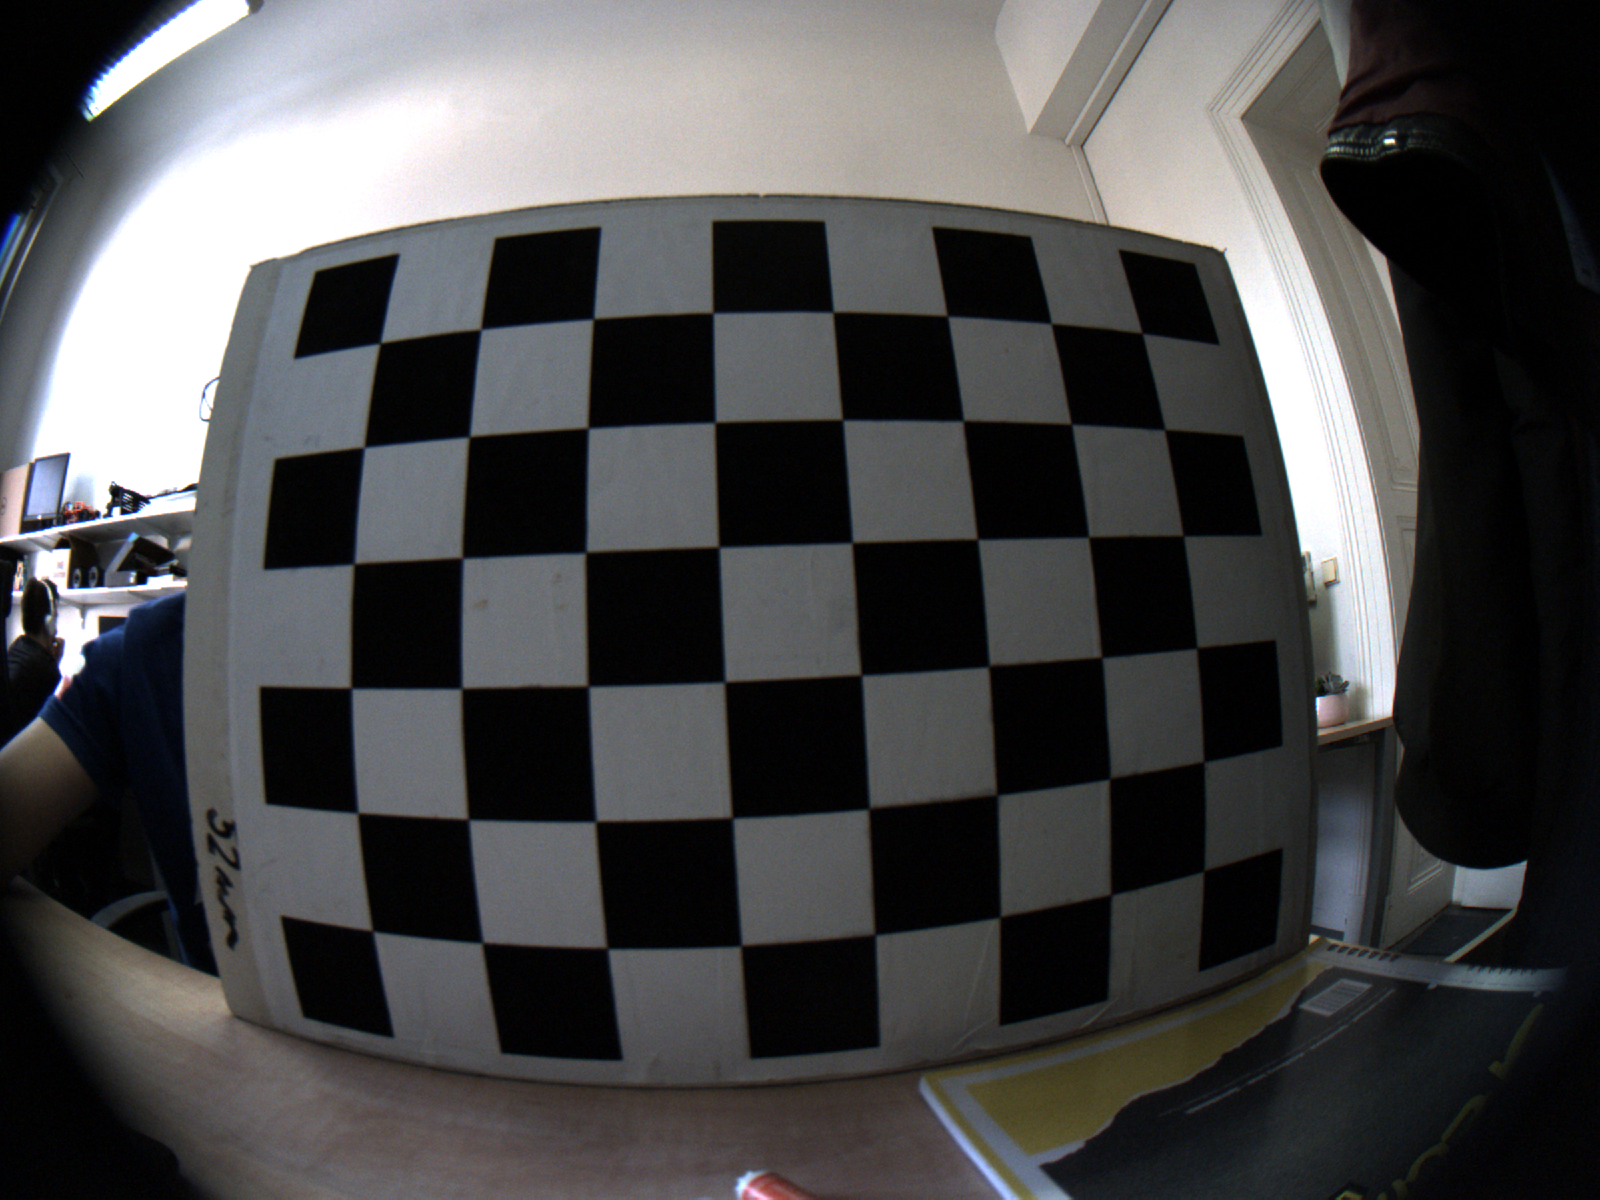
\includegraphics[width=\textwidth]{graphics/chessboard_img.png}
      \caption{Original image with radial distortion. Objects with straight edges appear curved in the image due to the distortion.}
      \label{fig:chb1}
    \end{subfigure}
    \hfill
    \begin{subfigure}[t]{0.45\textwidth}
      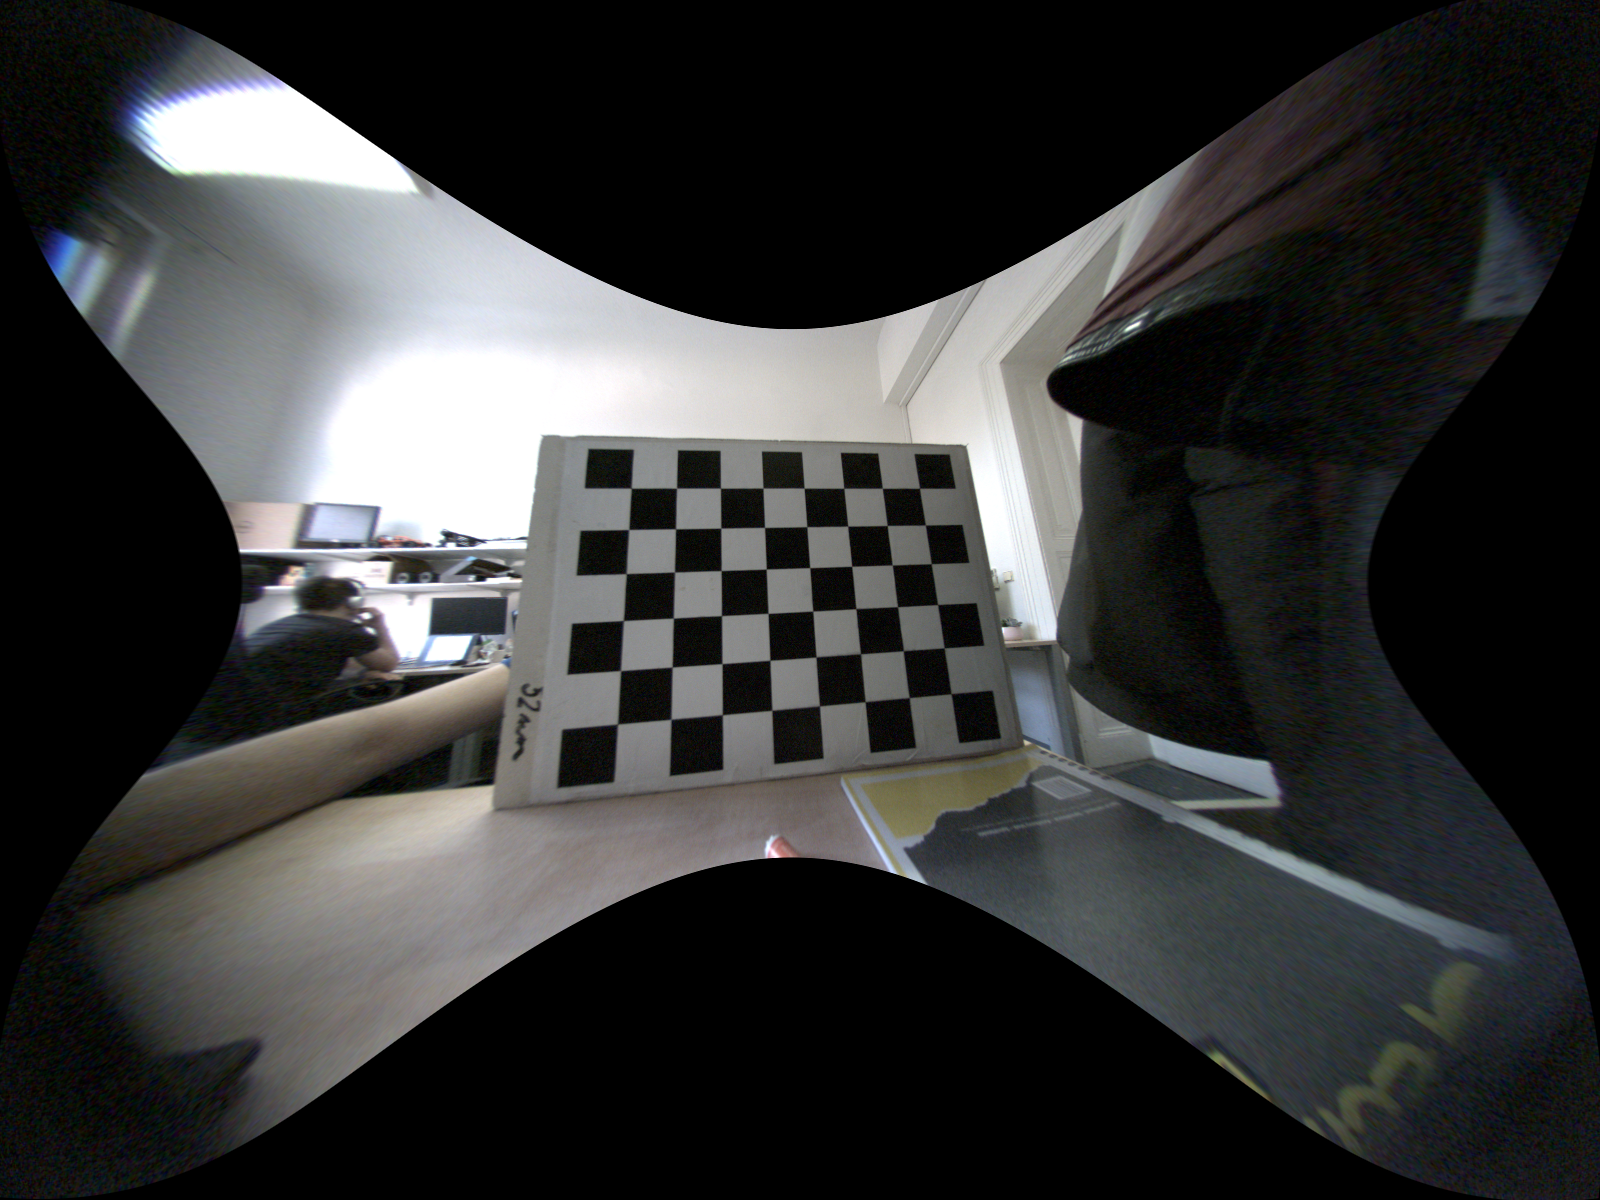
\includegraphics[width=\textwidth]{graphics/chessboard_img_rect.png}
      \caption{Image with no distortion. Edges that are straight in 3D are straight in the image.}
      \label{fig:chb2}
    \end{subfigure}
    \caption{An image from the camera before and after applying undistortion.}
    \label{fig:chb}
\end{figure}

Camera calibration is the process of empirically estimating the camera calibration matrix $\mat{K}$ (refer to eq. \eqref{eq:kmat}) and distortion parameters of the camera's optical system for the pinhole camera model described in \autoref{sec:pinhole_camera_model}.
Usually, this is done with some pattern with predefined parameters like a chessboard or more advanced markers (ChArUco and ArUco \cite{aruco} etc).

The camera calibration is necessary for geometrical image correction, distortion elimination, obtaining metric information, and further distance estimation (see \autoref{fig:chb}). 

In the real world, lenses have distortion (see \autoref{fig:chb1}).
To compensate that distortion, a polynomial model is often used with coefficients $k_1, ... , k_6$ for radial distortion and $p_1, p_2$ for tangential distortion.

\subsection{The minimal problem for camera calibration} 
It is the problem of obtaining a projection matrix $\mat{P}$ given $n=6$ correspondences of 3D scene points and 2D image points $\{(\vec{X}_i, \vec{m}_i)\}_{i=1}^n$.
Let the projection matrix $\mat{P}$ be 
\begin{equation}
    \label{eq:p_calib}
    \mat{P} = \begin{bmatrix}
        \vec{q}_1^\top & q_{14} \\
        \vec{q}_2^\top & q_{24} \\
        \vec{q}_3^\top & q_{34} \\
    \end{bmatrix}.
\end{equation}

The equation \eqref{eq:proj_min} can be expanded to
\begin{equation}
    \lambda_i u_i = \vec{q}_1^\top \vec{X}_i + q_{14}, \;\;\;
    \lambda_i v_i = \vec{q}_2^\top \vec{X}_i + q_{24}, \;\;\;
    \lambda_i = \vec{q}_3^\top \vec{X}_i + q_{34}, \;\;\;
\end{equation}
where $\vec{m}_i = \begin{bmatrix} u_i \\ v_i \end{bmatrix}$ is an image point, $ \lambda \in \mathbb{R}^{+}$, $i \in \{1, 2, ..., 6\}$.
After elimination of $\lambda_i$, we obtain
\begin{equation}
    (\vec{q}_3^\top \vec{X}_i + q_{34})u_i = \vec{q}_1^\top \vec{X}_i + q_{14},
\end{equation}
\begin{equation}
    (\vec{q}_3^\top \vec{X}_i + q_{34})v_i = \vec{q}_2^\top \vec{X}_i + q_{24}.
\end{equation}

\begin{equation}
    \label{eq:Aqmat}
    \mat{A} \vec{q} = \begin{bmatrix}
        \vec{X}_1^\top & 1 & \vec{0}^\top & 0 & -u_1 \vec{X}_1^\top & -u_1 \\
        \vec{0}^\top & 0 & \vec{X}_1^\top & 1 & -v_1 \vec{X}_1^\top & -v_1 \\ 
        \vdots & \vdots & \vdots & \vdots & \vdots & \vdots \\
        \vec{X}_k^\top & 1 & \vec{0}^\top & 0 & -u_k \vec{X}_k^\top & -u_k \\
        \vec{0}^\top & 0 & \vec{X}_k^\top & 1 & -v_k \vec{X}_k^\top & -v_k \\ 
    \end{bmatrix} \begin{bmatrix}
        \vec{q}_1 \\ q_{14} \\ \vec{q}_2 \\ q_{24} \\ \vec{q}_3 \\ q_{34}
    \end{bmatrix} = \vec{0},
\end{equation}
so for $k=6$, $\mat{A} \in \mathbb{R}^{12 \times 12}$, $\vec{q} \in \mathbb{R}^{12}$. If $\mat{A}$ has rank 12, there is no non-trivial null space for $\mat{A}$.

Equation \eqref{eq:Aqmat} can be solved by the so-called \textit{Jack-Knife estimation}. 
Let us denote a matrix $\mat{A}$ with the $i$-th row removed as $\mat{A}_i$. 
The \textit{Jack-Knife estimation} iterates through $i \in {1, \dots, 12}$.
In each iteration, if the right null-space of $\mat{A}_i$ is not empty, the matrix $\mat{P}_i$ can be decomposed to $\mat{K}_i$ $\mat{R}_i$ and $\vec{t}_i$.
Minimisation of the reprojection error from \autoref{sec:error_reprojection} for $i \in \{1, \dots, 12\}$ then can be used to find the best estimate of $\mat{P}$.

\subsection{Distortion correction}
After the matrix $\mat{P}$ is obtained, parameters of the distortion can be found as well.
The equation \eqref{eq:projection} can be rewritten using the relation from equation \eqref{eq:PKRt} as
\begin{equation}
    \label{eq:dist_start}
    \lambda \begin{bmatrix} 
        u \\ v \\ 1 \end{bmatrix} = \mat{K} [\mat{R} | \vec{t}] \begin{bmatrix} x \\ y \\ z \\ 1
    \end{bmatrix}.
\end{equation}
Let us now redefine this equation to consider the distortion. A 3D point in the camera frame can be expressed as 
\begin{equation}
    \label{eq:dist_2}
    \begin{bmatrix} x_c \\ y_c \\ z_c \end{bmatrix}
     = [\mat{R} | \vec{t}] \begin{bmatrix} x \\ y \\ z \\ 1
    \end{bmatrix}.
\end{equation}
The distortion model is then defined as 
\begin{equation}
    \label{eq:dist_3}
    x'' = \frac{x_c}{z_c} \frac{1 + k_1r^2 + k_2r^4 + k_3r^6}{1 + k_4r^2 + k_5r^4 + k_6r^6} + p_1(r + 2x') + 2p_2\frac{x_c y_c}{z^2_c},
\end{equation}
\begin{equation}
    \label{eq:dist_4}
    y'' = \frac{y_c}{z_c} \frac{1 + k_1r^2 + k_2r^4 + k_3r^6}{1 + k_4r^2 + k_5r^4 + k_6r^6} + 2p_1(\frac{x_c y_c}{z_c^2}) + p_2(r + 2y'),
\end{equation}
where $x' = (\frac{x_c}{z_c})^2$, $\;y' = (\frac{y_c}{z_c})^2$, $\;r = x' + y'$. Then, the corresponding undistorted point will be
\begin{equation}
    \label{eq:dist_end}
    \begin{bmatrix} u \\ v \\ 1 \end{bmatrix} = \mat{K} \begin{bmatrix} x'' \\ y'' \\ 1 \end{bmatrix}.
\end{equation}

Considering eq. \eqref{eq:kmat}, the image of a point $\vec{X}$ seen through the calibrated camera with a projection matrix $\mat{P}$ is obtained using eqs. \eqref{eq:dist_start} to \eqref{eq:dist_end}. 
Firstly, the point is projected to an abstract projection plane (eq. \eqref{eq:dist_2}). 
After that, distortion compensation is applied using the model described by equations \eqref{eq:dist_3} and \eqref{eq:dist_4}. 
Finally, the point is transformed from the metric system of the abstract projection plane to the image coordinate system (eq. \eqref{eq:dist_end}).

\section{General multicamera pose calibration}
\label{sec:stereocalib}

\begin{figure}[h]
    \centering
    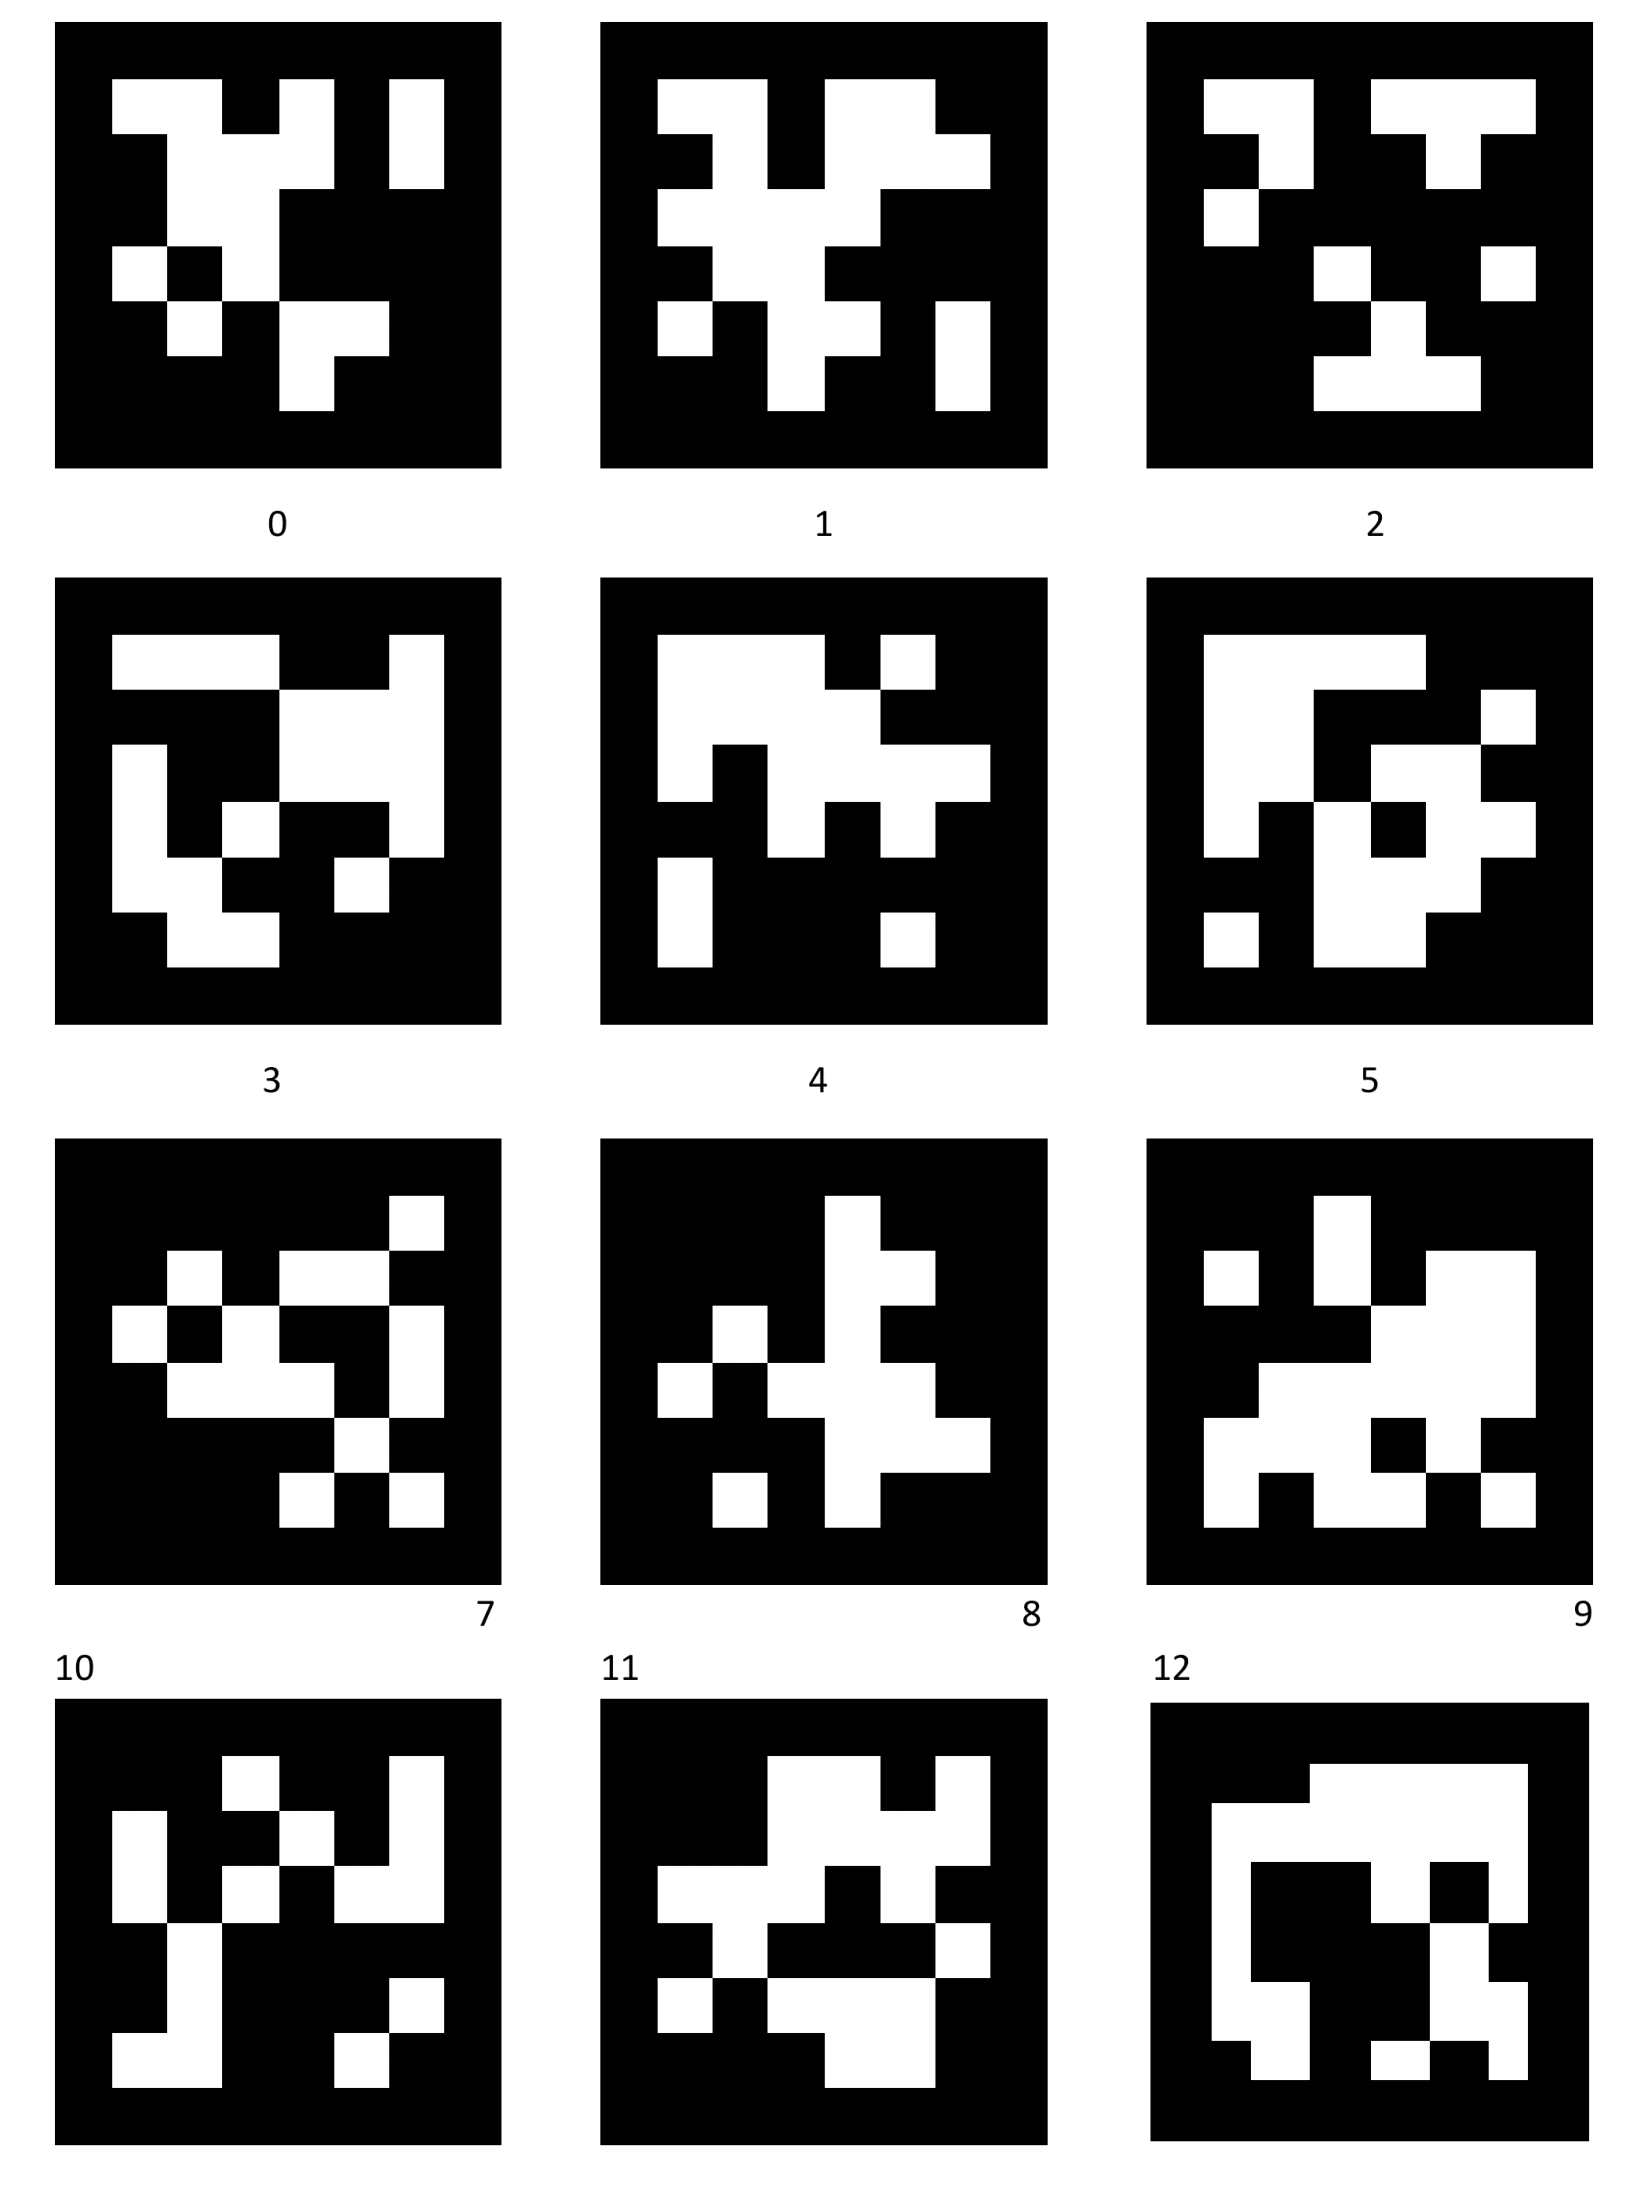
\includegraphics[width=.2\textwidth]{graphics/aptags.png}
    \caption[The calibration pattern using AprilTags.]{The calibration pattern using AprilTags that was used for the stereopair calibration.}
    \label{fig:aptags}
\end{figure}

Stereo pair calibration is a process of estimating the essential matrix $\mat{E}$ (defined in \autoref{sec:epipolar_geometry}) for a camera pair, which also expresses the relative rotation matrix $\mat{R}_{21}$ and relative translation vector $\vec{t}_{21}$ of a camera pair. 

There are multiple algorithms implementing stereo pair calibration.
Usually, a calibration pattern is used as the one shown in \autoref{fig:chb} for a standard stereo camera with parallel or converging optical axes.
Most algorithms assume that the whole pattern is seen in both images.
However, this is a disadvantage for cameras with a small overlapping zone and diverging optical axes.
For this reason, it is better to use some other pattern, for example, a set of AprilTags \cite{Malyuta2019} which can be detected separately. 
The pattern used in this work is shown in \autoref{fig:aptags}.

\subsection{Least-square estimation of transformation}
\label{sec:lsq_umeyama}
The first approach assumes that an initial estimate of the relative pose of the cameras is obtained using a manual measurement. 
The only necessary step is to correct the pose of one camera with respect to the other.
If there is no initial pose provided, the first camera pose is considered the world coordinate frame, and the relative transformation of the second camera is obtained. 
Firstly, corresponding parts of the calibration patterns are detected in $I_1$ and $I_2$, and their 3D positions are computed.
The AprilTag markers \cite{Malyuta2019} were used in this thesis, which also provides a unique identification of the markers and an estimate of their full relative pose.
In this way, two sets of 3D poses are obtained, each corresponding to the detected markers in one image.
Then, transformation parameters between the two point sets are estimated, and the correction transformation $\mat{T}_{c}$ is computed, where
\begin{equation}
    \mat{T}_{c} = 
    \begin{bmatrix}
        \mat{R}_c & \vec{t}_c \\ 
        0 & 1
    \end{bmatrix}.
\end{equation}

The algorithm is based on the analysis of the covariance matrix $\sum_{ab} \in \mathbb{R}^{3 \times 3}$ of the input sets $a$ and $b$.
It estimates parameters $\mat{R}_c$ and $\vec{t}_c$ such that
\begin{equation}
    \frac{1}{n} \sum_{i=1}^{n}{\lVert b_i - (\mat{R}_c a_i + \vec{t}_c) \rVert}^2
\end{equation}
is minimized, where $n$ equals to size of $a$ and $b$.
All details with derivation are available in \cite{Umeyama1991}.
A correct pose of the second camera then can be obtained by applying $\mat{T}_{c}$ to $\mat{R}_{21}$ and $\vec{t}_{21}$.

\subsection{PnP-based estimation of transformation}
\label{sec:pnp}
\begin{figure}[h]
    \centering
    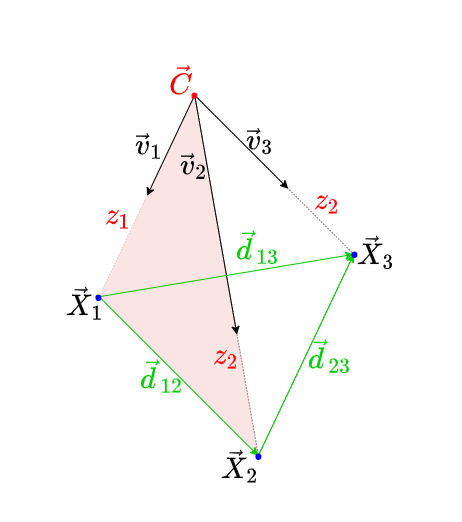
\includegraphics[width=.4\textwidth]{graphics/p3p.png}
    \caption[Visualization of the P3P problem.]{Visualization of the P3P problem. $\vec{C}$ is the camera center, vectors $\vec{v}_1$, $\vec{v}_2$ and $\vec{v}_3$ are vectors pointing to 3D points $\vec{X}_1$, $\vec{X}_2$, and $\vec{X}_3$, respectivly. The mutual position of the 3D points is known and expressed by vectors $\vec{d}_{12}$, $\vec{d}_{23}$, and $\vec{d}_{13}$. Scalars $z_1$, $z_2$, and $z_3$ are absolute distances from each 3D point to the camera center in world coordinate units (meters).}
    \label{fig:p3p}
\end{figure}

Another, the more general approach is based on solving a Perspective-n-Point (PnP) problem.
PnP is the problem of estimating a camera pose (translation and rotation) given a known set of $n$ 3D points and their respective 2D projections to an image of a calibrated camera.
Mathematically, the situation can be expressed as
\begin{equation}
    \label{eq:pnp_intro}
    \lambda_i \begin{bmatrix} \vec{m}_i \\ 1 \end{bmatrix} = \mat{K} \mat{R} (\vec{X}_i - \vec{C}), \;\; i \in \{0..n\}.
\end{equation}
No initial pose estimation is needed for this algorithm, but it can accelerate the solver if there is one.

\subsubsection{P3P}
The situation when $n=3$ is the minimal amount of points to solve the PnP problem.
This specific variant of PnP is called P3P.  
Firstly, let us define a vector $\vec{v}_i \in \mathbb{R}^3$ corresponding to a projection of a point in the image $\vec{m}_i$ as $\vec{v}_i = \mat{K}^{-1}\begin{bmatrix}\vec{m}_i \\ 1 \end{bmatrix}$. From eq. \eqref{eq:pnp_intro}, the following relation can be obtained:
\begin{equation}
    \label{eq:p3p_gen}
    \lambda_i \vec{v}_i = \mat{R} (\vec{X}_i - \vec{C}).
\end{equation}
If there is no rotation, the situation will look like in \autoref{fig:p3p} where vectors $\vec{d}_i$ are known, so eq. \eqref{eq:p3p_gen} simplifies to a system of three equations with three unknowns (vector $\vec{C}$).
If there is a non-zero rotation, it can be eliminated first.
Let us define a helper variable $z_i$ as the distance of a point $\vec{X}_i$ from $\vec{C}_i$:
\begin{equation}
    \label{eq:p3p_rot}
    |\lambda_i| \cdot \lVert \vec{v}_i \rVert = \lVert \vec{X}_i - \vec{C} \rVert = z_i.
\end{equation}
Considering only angles between $\vec{v}_i$ and applying the cosine law per $\triangle{\vec{C} \vec{X}_i \vec{X}_j}$, for $i, j \in \{1, 2, 3\}, i \neq j$, the relation
\begin{equation}
    \lVert \vec{d}_{ij} \rVert = z_i^2 + z_j^2 - 2z_iz_jc_{ij}
\end{equation}
may be obtained, where $\lVert \vec{d}_{ij} \rVert = \lVert \vec{X}_j - \vec{X}_i \rVert$, $c_{ij} = \cos(\angle \vec{v}_i \vec{v}_j)$.
After solving the system of three equations with three unknown $z_i$, there will be up to 4 solutions.
Each solution should be either verified on additional points \cite{Fischler1981} or sorted by reprojection error (refer \autoref{sec:error_reprojection}).
Having this, $\vec{C}$ can be found by trilateration (3 sphere intersection) from $\vec{X}_i$ and $z_i$; then $\lambda_i$ from eq. \eqref{eq:p3p_rot} and $\mat{R}$ from eq. \eqref{eq:p3p_gen}.

\subsubsection{P3P + RANSAC}
RANSAC stands for Random sample consensus. 
It is an iterative method of estimating the parameters of a model from a set of observed data that contains both inliers and outliers.
The more general PnP task can be solved as a combination of P3P and RANSAC algorithms.

At each iteration, 3 points out of $n$ are randomly sampled, and $\mat{R}$ and $\vec{t}$ are computed.
Then, the obtained transformation is confirmed on all $n$ points using the reprojection error described in \autoref{sec:error_reprojection}.
In the next iteration, the same process is repeated. 
If the maximum number of iterations is reached or the change in relative error is insufficient, $\mat{R}$ and $\vec{t}$, which provided the smallest error, are considered to be the result.

In practice, more sophisticated methods are employed, as in \cite{Lepetit2008, Hesch2011}.

\section{Feature extraction, matching and filtering}
\label{sec:features}
In computer vision, \textit{features} typically refer to representations of unique pieces of information from the image scene, such as points, edges, and objects.
A feature detector is an algorithm for extracting features from an image.
There are many such algorithms, but the ORB feature extractor is used in this thesis. 
The authors in \cite{Rublee2011} claim that ORB has comparable accuracy as the state-of-the-art SIFT detector while being a few times faster, which is also supported by other research \cite{Sharif2017}. 

The next step of the proposed method is mutually associating features in images from the two cameras, corresponding to the same physical objects in the environment. 
This is done by a feature matcher, which compares descriptors of the features provided by the feature detection algorithm.
Some feature matching algorithms perform a brute-force comparison of all combinations of features, others use nearest neighbors approximations or even neural networks \cite{Sarlin2020}.

A brute-force matcher is one of the simplest matchers, and it is used in the proposed solution.
It takes one descriptor from one set, computes its similarity to all descriptors from the second set, and matches it with the most similar feature. 
This process is repeated to maximize the overall similarity between the two sets.

Even after this process, there are typically some outliers.
Distance from features to the corresponding epipolar lines can be used to filter them. 
This distance can be computed using the equation \eqref{eq:epiconstr}.
If the distance of the matched feature from the corresponding epipolar line in the other image is larger than a specified threshold, the match is dismissed as an outlier.

\section{Feature position estimation}
Positions of the observed 3D points in the scene can be computed from pairs of correspondent points taken by calibrated cameras with a known relative pose.
This process is called triangulation.
Correspondences for triangulation are received as a result of feature detection, matching, and filtering.

\subsection{Shortest distance triangulation}
\label{sec:shortest_distance}
One triangulation method is based on finding the shortest distance between two rays.
According to the epipolar geometry properties described in \autoref{sec:epipolar_geometry} and visualized in \autoref{fig:epipolar_std}, vectors $\vec{d}_1$ and $\vec{d}_2$ intersects at the 3D point $\vec{X}$.
However, in the real world, the rays can be at some distance from each other due to imperfect stereo pair calibration, so $\vec{X}$ is estimated as the point closest to both lines.

It is possible to compute $\vec{d}_1$ and $\vec{d}_2$ in a common coordinate frame from $\vec{m}_1$ and $\vec{m}_2$, since the relative pose of the cameras is known.
Then, let us define two lines $d_1$ and $d_2$ in a vector form:
\begin{equation}
    \label{eq:shortest_d1}
    d_1: \vec{p}_1 = \vec{C}_1 + t \vec{d}_1,
\end{equation}
\begin{equation}
    \label{eq:shortest_d2}
    d_2: \vec{p}_2 = \vec{C}_2 + s \vec{d}_2,
\end{equation}
where $\vec{d}_1$ and $\vec{d}_2$ are directional vectors, $\vec{C}_1$ and $\vec{C}_2$ are 3D points located on the respective lines (camera centers in this case), $s \in \mathbb{R}$ and $t \in \mathbb{R}$ are free parameters that uniquely define points $\vec{p}_1$ and $\vec{p}_2$. 
Distance between the two lines is minimal at the point where the vector $\vec{l} = \vec{p}_2 - \vec{p}_1$ is orthogonal to $d_1$ and $d_2$, which can be expressed using a dot product as 
\begin{equation}
    \label{eq:ldd1}
    \vec{l} \cdot \vec{d}_1 = 0,
\end{equation}
\begin{equation}
    \label{eq:ldd2}
    \vec{l} \cdot \vec{d}_2 = 0.
\end{equation}
After substituting eqs. \eqref{eq:shortest_d1} and \eqref{eq:shortest_d2} to these equations, a system of two equations with two unknowns $s$ and $t$ is obtained.
This system has a unique solution unless the rays are parallel.
Using $s$ and $t$, the points $\vec{p}_1$ and $\vec{p}_2$ can be obtained and then $\vec{X}$ is calculated as $\vec{X} = \frac{\vec{p}_1 + \vec{p}_2}{2}$.

\subsection{SVD triangulation}
\label{sec:svdtriang}
Triangulation using Singular Value Decomposition (SVD) is another method that is more precise and widely used.
It computes 3D points from 2D correspondences using the camera matrices $\mat{P}_1$, $\mat{P}_2$. 
This method is derived and described in detail in \cite{hartley_zisserman_2004}, p.312. Here, a short summary is provided.

The projection equation \eqref{eq:projection} can be rewritten as
\begin{equation}
    \lambda_i \begin{bmatrix} 
        u_i \\ v_i \\ 1 \end{bmatrix} = \mat{P}_i
    \begin{bmatrix} \vec{X} \\ 1
    \end{bmatrix},
\end{equation} 
where $\mat{P}_i$ decomposes as in eq. \eqref{eq:p_general}, and $\lambda_i \neq 0$, $i \in \{1, 2\}$.
After eliminating $\lambda_1$, $\lambda_2$ we obtain the following set of equations:
\begin{equation}
    \mat{D} \begin{bmatrix} \vec{X} \\ 1 \end{bmatrix} = \vec{0}, \;\;\;\;\;
    \mat{D} = \begin{bmatrix}
        u_1 (\vec{p}_{1, 3})^\top - (\vec{p}_{1, 1})^\top \\
        v_1 (\vec{p}_{1, 3})^\top - (\vec{p}_{1, 2})^\top \\
        u_2 (\vec{p}_{2, 3})^\top - (\vec{p}_{2, 1})^\top \\
        v_2 (\vec{p}_{2, 3})^\top - (\vec{p}_{2, 2})^\top \\
    \end{bmatrix}, \;\;\;\;\; \mat{D} \in \mathbb{R}^{4 \times 4}.
\end{equation}

The result of the triangulation is the eigenvector corresponding to the smallest eigenvalue.
The eigenvectors and eigenvalues are obtained using $\mathsf{SVD}$ decomposition of $\mat{D}^\top\mat{D}$, which is a solution of an equation
\begin{equation}
    \mat{U}\mat{S}\mat{V}^\top = \mat{D}^\top\mat{D},
\end{equation}
where $\mat{U}$ and $\mat{V}$ are orthogonal matrices and $\mat{S}$ is a non-negative diagonal matrix.

Let the eigenvector corresponding to the smallest eigenvalue as $\vec{h} = (x', y', z', w')^\top$.
The triangulated point then can be expressed as
\begin{equation}
    \vec{X} = \begin{bmatrix}
        \frac{x'}{w'} \\
        \frac{y'}{w'} \\
        \frac{z'}{w'} \\
    \end{bmatrix}.
\end{equation}

The improved version of this algorithm called "The Golden Standard Triangulation Method" is more widely used in practice.
It combines SVD triangulation with Sampson correction (description is available in \cite{hartley_zisserman_2004}, p. 314). 
